\chapter{Quantization}

As mentioned in the introduction, two operations are necessary to transform an analog waveform into a digital signal.
The first action, discussed in Chapter~\ref{chapter:FourierAnalysisSampling}, is called sampling.
It consists of converting a continuous-time input into a discrete-time signal.
The second operation is the process of approximating continuous-space samples by a discrete set of possible symbols.
This process termed \emph{quantization} is equally essential in order to transmit an analog signal over digital media.
Quantization invariably induces a loss in signal quality.
The \emph{distortion} between the original and quantized signals is usually unwanted, and cannot be reversed.
Yet, for a specific application, the level of signal degradation can be controlled.


\section{Scalar Quantizers}

Generic quantizers operate on large classes of signals and are very robust.
In scalar quantization, each source value is processed individually, with the quantizer output taking one of finitely many possibilities.
The number of quantization levels tends to be a base-two exponent because the output of the quantizer is often represented using binary symbols.
Mathematically, a quantizer can be expressed as a function.
Suppose that the input to the quantizer is a real number, and its output is a value that belongs to the set $\mathcal{Q}$.
Then we can describe the quantizer as a function $Q : \mathbb{R} \mapsto \mathcal{Q}$ with output
\begin{equation*}
x_{\mathrm{q}} = Q(x) .
\end{equation*}
This is perhaps best seen through an example.


\begin{example}
Let $Q : \mathbb{R} \mapsto \mathcal{Q}$ be a quantizer with four possible outputs labeled $q_1$ through $q_4$.
The output $x_{\mathrm{q}}$ of the quantizer belongs to set $\mathcal{Q}$, and it must therefore be equal to one of the four possible pointslisted above.
Figure~\ref{figure:Quantizer} shows the functional representation of a four-level quantization scheme.
\begin{figure}[htbp]
\begin{center}
\begin{psfrags}
\psfrag{q1}[l]{$q_1$}
\psfrag{q2}[l]{$q_2$}
\psfrag{q3}[l]{$q_3$}
\psfrag{q4}[l]{$q_4$}
\psfrag{o}[c]{Output}
\psfrag{i}[c]{Input}
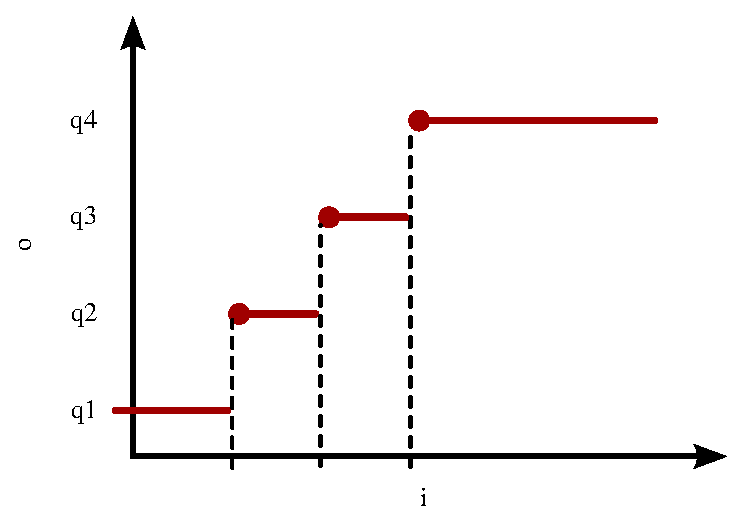
\epsfig{file=Figures/quantizer,width=6cm}
\end{psfrags}
\caption{A functional representation of a quantizer.}
\label{figure:Quantizer}
\end{center}
\end{figure}

The output of the quantizer in this example is determined according to a nearest neighbor rule.
Note that this function is not injective (one-to-one) and, as such, has no inverse.
\end{example}


\section{Distortion Measures}

To compare different quantizers, a performance metric must be established.
A common distortion criterion with nice properties is the square of the error
\begin{equation} \label{equation:QuantizationErrorSquared}
d(x, x_{\mathrm{q}}) = (x - Q(x))^2 = e_{\mathrm{q}}^2 ,
\end{equation}
where $e_{\mathrm{q}} = x - x_{\mathrm{q}}$ is the \emph{quantization error}.
The criterion in \eqref{equation:QuantizationErrorSquared} specifies how close the output $x_{\mathrm{q}}$ is to $x$ for a specific realization of $x$.
Since the quantizer is designed to operate on an information signal, a more relevant assessment of performance weighs in the accuracy of the quantizer over all possible realizations of the input.
An appropriate distortion measure for the quantization of a random signal is provided by the \emph{mean squared error (MSE)},
\begin{equation} \label{equation:QuantizationMSE}
\mathrm{E} [ d(x, x_{\mathrm{q}}) ]
= \mathrm{E} [(x - Q(x))^2 ] = \| e_{\mathrm{q}} \|^2 .
\end{equation}
Note that this performance metric depends on the distribution of the input signal, and hence is tied to a specific application.
A quantizer can be said to work well in a particular context.
However, describing the performance of a quantization scheme without specifying the properties of its input signal is meaningless.

\begin{example} \label{example:UniformQuantizer}
Suppose that the values of a discrete-time information signal are uniformly distributed over $[0,16]$.
Furthermore, assume that the quantizer implements a nearest neighbor rule with quantization levels equal to $q_i = 2i - 1$ for $i = 1, 2, \ldots, 8$.
We wish to find the mean squared error of this quantization scheme.

Being uniformly distributed, the probability density function of the input signal is
\begin{equation*}
f_x (\xi) = \frac{1}{16}
\end{equation*}
for $\xi \in [0, 16]$, and zero otherwise.
The decision regions corresponding to the various quantization points are then given by $[0, 2], (2, 4], \ldots, (14, 16]$.
We can therefore compute the mean squared error as follows,
\begin{equation*}
\begin{split}
\mathrm{E} [ d(x, x_{\mathrm{q}}) ]
&= \mathrm{E} [(x - Q(x))^2 ]
= \int_0^{16} \frac{(\xi - Q(\xi))^2}{16} d\xi \\
&= \sum_{i=1}^8 \int_{2i-2}^{2i} \frac{(\xi - (2i - 1))^2}{16} d\xi \\
&= \frac{1}{2} \int_{0}^{2} (\xi + 1)^2 d\xi = \frac{1}{3} .
\end{split}
\end{equation*}
That is, the mean square error associated with this input distribution and quatization scheme is $\| e_{\mathrm{q}} \|^2 = \frac{1}{3}$.
\end{example}

One of the criticisms about the MSE of \eqref{equation:QuantizationMSE} is that it has a tendency to assign a larger distortion value to signal input with sizable second moments.
Indeed, an information process likely to feature large amplitudes is bound to yield outputs with a large mean squared error.
On the other hand, under this absolute metric, most quantizers may appear to work well for minute signals as their mean square errors are destined to remain small.
An alternative and closely related criterion that takes into consideration the power of the original signal is the \emph{signal-to-quantization-noise ratio (SQNR)},
\begin{equation} \label{equation:SQNR}
\text{SQNR} = \frac{\| x \|^2}{\| e_{\mathrm{q}} \|^2}
= \frac{\mathrm{E} [ x^2 ]}{\mathrm{E} [(x - Q(x))^2 ]} .
\end{equation}
Because of the implicit normalization associated with \eqref{equation:SQNR}, this latter performance measure is more suitable to compare quantizer performance for different input processes.

\begin{example}
This time, assume that the values of a discrete-time information signal are uniformly distributed over $[0,2]$.
To avoid confusion, we denote the input signal in the present problem using $y$.
We wish to obtain the mean squared error associated with the quantizer of Example~\ref{example:UniformQuantizer}, applied to the signal at hand.
Also, we wish to compare the SQNR of the quantization scheme of Example~\ref{example:UniformQuantizer} with the SQNR of the scenario described in this example.

To derive the mean squared error, we follow the same steps as before
\begin{equation*}
\begin{split}
\mathrm{E} [ d(y, y_{\mathrm{q}}) ]
&= \int_0^{2} \frac{(\zeta - Q(\zeta))^2}{2} d\zeta \\
&= \frac{1}{2} \int_{0}^{2} (\zeta - 1)^2 d\zeta = \frac{1}{3} .
\end{split}
\end{equation*}
We notice that the MSE is the same as the one derived in Example~\ref{example:UniformQuantizer}.
Nevertheless, the quantization scheme seems more suited to the signal described in the previous example.
The SQNR of the current scheme is given by
\begin{equation*}
\text{SQNR} = \frac{\| y \|^2}{\mathrm{E} [ d(y, y_{\mathrm{q}}) ]}
= 3 \| y \|^2 = 4.
\end{equation*}
This can be compared with the SQNR of the problem featured in Example~\ref{example:UniformQuantizer}, which is given by
\begin{equation} \label{equation:UniformQuantizerSQNR}
\text{SQNR} = \frac{\| x \|^2}{\mathrm{E} [ d(x, x_{\mathrm{q}}) ]}
= 3 \| x \|^2 = 256.
\end{equation}
Obvioulsy, the SQNR is much better in the case of Example~\ref{example:UniformQuantizer}.
Can you think of an eight-level quantization scheme that would perform better for the current problem, perhaps rivaling the SQNR of \eqref{equation:UniformQuantizerSQNR}?
\end{example}

Both the mean squared error and the signal-to-quantization-noise ratio are valid and meaningful ways to present performance results for quantization schemes.
Still, they must be put in proper context, especially when comparing scenarios where the distributions of the input signals differ.
For a fixed input process, a quantization scheme that minimizes the MSE will invariably maximize the SQNR.


\section{Uniform Quantizers}

Finding an optimal quantizer is not an easy task.
An eight-level quantizer has eight degrees of freedom, and the overall performance of the quantizer is jointly determined by the positions of the quantization points.
A means to reduce the difficulty of identifying an optimal quantization scheme is to constraint the possible candidates.
This can be achieved, for instance, by imposing a rule on the respective position of the quantization points.
Restricting the search space to uniform quantizers is one possible way to ensure that an optimal quantizater can be found.

A \emph{uniform quantizer} is a function where the locations of successive outputs are situated at a fixed interval, $q_i - q_{i-1} = \Delta$ for all the possible values.
It is one of the simplest quantizer designs.
The quantization scheme considered in Figure~\ref{figure:Quantizer} is in fact a uniform quantizer.
The distance between two quantization points is the same for all neighbors.
If the objective function of the optimization process is the mean squared error, then optimal locations for the quantization points can be found in a straightforward manner.
First, note that we can write the postion of the quantization points as
\begin{equation*}
q_i = q_1 + (i-1) \Delta
\end{equation*}
for $i = 1, 2, \ldots, \ell$ where $\ell$ is the number quantization levels.
As usual, the MSE is given by
\begin{equation*}
\mathrm{E} [ d(x, x_{\mathrm{q}}) ]
= \int_{-\infty}^{\infty} (\xi - Q(\xi))^2 f_x(\xi) d\xi .
\end{equation*}
We emphasize  that the performance of the quantizer is optimize by minimizing the value of the integrant at each point.
We deduce that the decision regions corresponding to $q_1, q_2, \ldots, q_{\ell}$ must be equal to
\begin{equation*}
\left( - \infty, q_1 + \frac{\Delta}{2} \right],
\left( q_2 - \frac{\Delta}{2}, q_2 + \frac{\Delta}{2} \right],
\ldots,
\left( q_{\ell} - \frac{\Delta}{2}, \infty \right) ,
\end{equation*}
respectively.
The objective function then becomes
\begin{equation} \label{equation:UniformQuantizerMSE}
\begin{split}
\text{MSE} &= \int_{-\infty}^{q_1 + \frac{\Delta}{2}} (\xi - q_1)^2 f_x(\xi) d\xi
+ \sum_{i=2}^{{\ell}-1}
\int_{q_i - \frac{\Delta}{2}}^{q_i + \frac{\Delta}{2}}
(\xi - q_i)^2 f_x(\xi) d\xi \\
&+ \int_{q_{\ell} - \frac{\Delta}{2}}^{\infty} (\xi - q_{\ell})^2 f_x(\xi) d\xi .
\end{split}
\end{equation}
The resulting optimization process now has two degrees of freedom, namely $q_1$ and $\Delta$.
For a suitable probability density function $f_x(\cdot)$, an optimal solution can be obtained explicitly using standard optimization methods.

\begin{example}
We revisit Example~\ref{example:UniformQuantizer} in the context of uniform quantizers.
Again, suppose that the values of the discrete-time input process are uniformly distributed over $[0, 16]$.
We wish to find the optimal eight-level uniform quantizer associated with this input distribution.

For simplicity, we assume that the quantization points $\{ q_1, q_2, \ldots, q_8 \}$ are contained in the interval $[0, 16]$.
This implies that $q_1 > 0$ and $q_8 < 16$.
The mean squared error as a function of $q_1$ and $\Delta$ is given by \eqref{equation:UniformQuantizerMSE}, which becomes
\begin{equation*}
\begin{split}
\text{MSE}~(q_1, \Delta)
%&= \int_{0}^{q_1 + \frac{\Delta}{2}} \frac{(\xi - q_1)^2}{16} d\xi
%+ \sum_{i=2}^{7}
%\int_{q_i - \frac{\Delta}{2}}^{q_i + \frac{\Delta}{2}}
%\frac{(\xi - q_i)^2}{16} d\xi
%+ \int_{q_8 - \frac{\Delta}{2}}^{16} \frac{(\xi - q_8)^2}{16} d\xi \\
&= \int_{-q_1}^{\frac{\Delta}{2}} \frac{\xi^2}{16} d\xi
+ 6 \int_{- \frac{\Delta}{2}}^{\frac{\Delta}{2}} \frac{\xi^2}{16} d\xi
+ \int_{- \frac{\Delta}{2}}^{16 - q_8} \frac{\xi^2}{16} d\xi \\
\end{split}
\end{equation*}
Recall that, by construction, we can write $q_8 = q_1 + 7 \Delta$.
Taking first derivatives with respect to $q_1$ and $\Delta$, we obtain
\begin{align*}
\frac{\partial}{\partial q_1} \text{MSE}~(q_1, \Delta)
&= \frac{q_1^2}{16} - \frac{(16 - q_1 - 7 \Delta)^2}{16} \\
\frac{\partial}{\partial \Delta} \text{MSE}~(q_1, \Delta)
&= \frac{7 \Delta^2}{64} - \frac{7 (16 - q_1 - 7\Delta)^2}{16} .
\end{align*}
Setting these derivatives equal to zero, we get $q_1 = 1$ and $\Delta = 2$.
A second derivative test ensures that this corresponds to a local minimum.
Since this point is the only stationary point of the function $\text{MSE}~(q_1, \Delta)$ within our search space, we gather that the quantization scheme of Example~\ref{example:UniformQuantizer} coincide with the optimal uniform quantizer.
\end{example}





\newpage

A quantizer can work either on single-source outputs or on blocks of source outputs.
Although more complex, the latter approach typically yields better performance.

\section{Lloyd-Max Algorithm}


\section{Analysis-Synthesis Coders}


